
\section{Organisation}

\begin{frame}
  {Literatur | Einführungen}
  \onslide<+->
  \onslide<+->
  Die folgenden drei Bücher sind die Grundlage des Seminars:\\
  \Zeile
  \begin{itemize}[<+->]
    \item \alert{\citet{ChierchiaMcconnellginet2000}} | GB-orientiert, nur die Kapitel von Chierchia
    \item \alert{\citet{DowtyEa1981}} | Tolle Montague-Einführung von seinen Schülern
    \item \alert{\citet{ParteeEa1990}} | Wichtige Grundlagen (Algebra, Logik), viele Druckfehler
  \end{itemize}
  \onslide<+->
  \centering 
  \large
  \Zeile
  \rot{Die auf den Folien angegebenen Teile dieser Bücher sollten\\
  für die Prüfungen durchgearbeitet werden. Das heißt natürlich nicht,\\
  dass Sie alles auswendig lernen sollen. Die Folien geben die Hinweise,\\
  was aus den Texten wichtig ist, sind aber nicht selbsterklärend.}
\end{frame}

\begin{frame}
  {Literatur | weitere Empfehlungen}
  \onslide<+->
  \begin{itemize}[<+->]
    \item \alert{\citet{Bucher1998}} | Lesbare Logik-Einführung auf Deutsch
    \item \alert{\citet{Carpenter1997}} | Prima Hardcore-Einführung mit Kategorialgrammatik
    \item \alert{\citet{Gutzmann2019}} | Aktuelle Einführung auf Deutsch
  \end{itemize}
\end{frame}


\begin{frame}
  {Seminarverlauf}
  \onslide<+->
  \begin{enumerate}[<+->]\Lf\scriptsize
    \item \alert{9.10.2023} Diskussion: Wie schlussfolgern wir? Wie hängen unsere Schlussfolgerungen mit Semantik zusammen?
    \item \alert{26.10.2023} Referentielle Semantik (Folien 2)
    \item \alert{02.11.2023} Referentielle Semantik (Folien 2) II
    \item \alert{09.11.2023} Mengen- und Funktionstheorie (Folien 3)
    \item[\rule{1.2em}{1.2em}] \raisebox{2pt}{\grau{16.11.2023 Ausfall wegen Dienstreise}}
    \item \alert{23.11.2023} Aussagenlogik (Folien 4)
    \item \alert{30.11.2023} Prädikatenlogik (Folien 5)
    \item \alert{07.12.2023} Quantifikation und modelltheoretische Semantik (Folien 6)
    \item \alert{14.12.2023} Getypte λ-Sprachen höherer Ordnung (Folien 7)
    \item \alert{21.12.2023} Intensionalität (Folien 8)
    \item[\rule{1.2em}{1.2em}] \raisebox{2pt}{\grau{28.12.2023 Weihnachtsferien}}
    \item[\rule{1.2em}{1.2em}] \raisebox{2pt}{\grau{04.01.2024 Weihnachtsferien}}
    \item \alert{11.01.2024} Tempus und Modalität (Folien 9)
    \item \alert{18.01.2024} Montagues intensionale Logik (Folien 10)
    \item \alert{25.01.2024} Lektüre 
    \item \alert{01.02.2024} Lektüre
    \item \alert{08.02.2024} Lektüre
  \end{enumerate}
\end{frame}

\begin{frame}
  {Semesterplan und Lernen für die Prüfung}
  \onslide<+->
  \onslide<+->
  \centering 
  \alert{\large Hinweis in eigener Sache}\\
  \Halbzeile
  \begin{itemize}[<+->]
    \item Vermutlich ist der Plan bis Weihnachten zu ambitioniert.
    \item Die Wochen 4 und 5 könnten länger dauern, Woche 7 ebenfalls.
    \item Dann ändert sich der Plan noch, eventuell fliegen Artikel am Ende raus.
  \end{itemize}
  \Zeile
  \onslide<+->
  \alert{\large Hinweis zum Lernen}\\
  \Halbzeile
  \begin{itemize}[<+->]
    \item Wir haben es hier mit anspruchsvollem Material zu tun.
    \item Nur so ergibt meiner Meinung nach formale Semantik Sinn,\\
      und irgendwelche weichgespülten Einführungen sind grob fahrlässig.
    \item Daher gilt aber: Wenn Sie nicht von Anfang an lernen,\\
      wird es sehr wahrscheinlich gegen Ende sehr schwierig!
  \end{itemize}
\end{frame}

\begin{frame}
  {Prüfungen}
  \onslide<+->
  \onslide<+->
  Einheitlicher Inhalt für alle Modul- und Examensprüfungen:\\
  \Zeile
  \begin{enumerate}[<+->]
    \item eine oder zwei inhaltliche Fragen zu den Themen der \textit{Sprachphilosophie}\\
      \grau{\footnotesize Die Liste der relevanten Texte wird rechtzeitig vor den Prüfungen eingeschränkt.}
    \item eine Logik-Aufgabe (natürliche Deduktion) -- \alert{außer in mündlichen Prüfungen}
    \item eine Semantik-Aufgabe (kompositionale Modellierung eines Satzes)
  \end{enumerate}
  \Zeile
  \onslide<+->
  \grau{Hausarbeiten nach Absprache.}
\end{frame}

\begin{frame}
  {Die unausweichliche Frage nach ein paar Wochen \visible<2->{| \rot{WTF???}}}
  \onslide<+->
  \onslide<+->
  \onslide<+->
  "`Wozu brauchen wir das denn?"'\\
  \Halbzeile
  \begin{itemize}[<+->]
    \item Nicht zu leugnende \alert{logische Eigenschaften von Sprache}
    \item Kleiner Einblick in deren \alert{technisch sehr aufwendige Beschreibung}
      \Halbzeile
    \item Wichtige Lernziele
      \begin{itemize}[<+->]
        \item Realistische Einschätzung \alert{eigener semantischer Intuitionen}
        \item Erkennen der \alert{Grenzen der Möglichkeiten von Logik} in der Analyse von Sprache
        \item Für zukünftige Forschende | \alert{Grundausbildung in formaler Semantik unabdinglich}
      \end{itemize}
  \end{itemize}
\end{frame}

\section{Schlussfolgern}

\begin{frame}
  {Was folgt logisch?}
  \onslide<+->
  \onslide<+->
  Fallen Ihnen logische Schlussfolgerungen aus diesen Aussagen ein?\\
  \Halbzeile
  \begin{itemize}[<+->]
    \item Das Semester hat begonnen.
    \item Olha hat einen sehr leichten ukrainischen Akzent.
    \item Entweder regnet es gerade, oder die Wasserleitung ist gebrochen.
    \item Es regnet, oder die Wasserleitung ist gebrochen. Es regnet seit zwei Stunden.
    \item Falls der Dänemark-Urlaub ausfällt, fahre ich eine Woche zu meinen Eltern.\\
      Der Dänemark-Urlaub fällt aus.
    \item Wenn es regnet, wird die Straße nass. Die Straße ist nicht nass.
    \item Es ist nicht der Fall, dass der WANG PC keine Festplatten unterstützt hat.
  \end{itemize}
\end{frame}

\begin{frame}
  {Folgt B aus A?} % Sätze
  \onslide<+->
  \begin{itemize}[<+->]
    \item A: Ein blauer Renault fährt auf der A9 Richtung Berlin.\\
      \alert{B: Ein Renault fährt auf der A9 Richtung Berlin.}
    \item A: Ich finde Geranien abstoßend.\\
      \alert{B: Ich habe schon mindestens einmal mindestens eine Geranie gesehen.}
    \item A: Der WANG PC ist nicht IBM-kompatibel.\\
      \alert{B: Es existiert mindestens ein WANG PC.}
    \item A: Alle Menschen sind intelligent.\\
      \alert{B: Horst Lichter ist intelligent.}
    \item A: Krister hat mir seinen Volvo Amazon verkauft.\\
      \alert{B: Irgendjemand hat seinen Volvo Amazon verkauft.}
  \end{itemize}
\end{frame}

\begin{frame}
  {Folgt B aus A?} % Lexik und Grammatik
  \begin{itemize}[<+->]\small
    \item A: Entweder regnet es, oder die Wasserleitung im Bad ist gebrochen, und die Wasserleitung im Bad ist gebrochen.\\
      \alert{B: Es regnet nicht.}
    \item A: Michelle hat uns den Dobermann für eine Woche zur Pflege überlassen.\\
      \alert{B: Der Dobermann wurde uns für eine Woche zur Pflege überlassen.}
    \item A: Jan glaubt, dass seine Sendung nicht abgesetzt wird.\\
      \alert{B: Jan glaubt nicht, dass seine Sendung abgesetzt wird.}
    \item A: Falls Dr.\ Kohl jetzt wieder Kanzler der BRD ist, gibt es vermutlich jeden Tag Pfälzer Saumagen zum Abendessen.\\
      \alert{B: Es gibt einen Kanzler der BRD.}
    \item A: Ein Mensch betritt den Raum.\\
      \alert{B: Es gibt mindestens einen Menschen.}
    \item A: Ein Mensch, der die Bibel gelesen hat, begeht im Durchschnitt nicht weniger Straftaten als andere.\\
      \alert{B: Es gibt mindestens einen Menschen.}
    \item A: \textit{We don't need no education.}\\
      \alert{B: Yes, you do! You just used a double negative.}
  \end{itemize}
\end{frame}

\begin{frame}
  {Folgt B aus A?} % Stories
  \onslide<+->
  \begin{itemize}[<+->]
    \item A: Herr Keydana fährt einen Golf. Alles, was einen Golf fährt, ist entweder menschlich oder eine AI, die auf Deep Learning basiert. Es gibt keine AI, die auf Deep Learning basiert, die einen Golf fährt.\\
      \alert{B: Es gibt mindestens einen Menschen.}
      \Halbzeile
    \item A: Es gibt an der Uni Göttingen mindestens einen Dozenten, der einen Golf fährt. Götz ist Dozent an der Uni Göttingen und Radsportler. Sein Auto ist gerade in der Werkstatt. Jeder Dozent an der Uni Göttingen fährt entweder einen Golf oder ist kein Radsportler, falls sein Auto in der Werkstatt ist.\\
      \alert{B: Götz fährt einen Golf.}
  \end{itemize}
\end{frame}

\begin{frame}
  {Logik}
  \onslide<+->
  \onslide<+->
  \centering 
  Versuchen Sie, eine Definition des Begriffs \alert{logische Schlussfolgerung} zu geben.\\
  \onslide<+->
  \Zeile
  Wann folgt eine Aussage aus einer oder mehreren anderen Aussagen?
\end{frame}

\begin{frame}
  {Inferenz | Abduktion}
  \onslide<+->
  \onslide<+->
  Entspricht oft der "`Alltagslogik"'. Suche nach \alert{spontan plausiblen Ursachen}.\\
  \Halbzeile
  \begin{itemize}[<+->]
    \item A: Der Verdächtige hat kein Alibi und ein Motiv.\\
      B: Der Verdächtige ist der Täter.
    \item Ich habe so einen komischen Husten, und die Infektionszahlen steigen wieder.\\
      B: Oh mein Gott, ich habe Covid!
    \item A: Es soll eine Impfpflicht eingeführt werden.\\
      B: George Soros und Bill Gates wollen uns Mikrochips einpflanzen.
    \item A: In Mikes Büro ist um 22 Uhr noch Licht.\\
      B: Mike bereitet seine Lehrveranstaltung für morgen vor.
  \end{itemize}
  \onslide<+->
  \centering 
  \Zeile 
  \orongsch{Hochgradig gefährlich, weil nicht formalisierbar und sehr bequem.}\\
  \alert{Gleichzeitig im Alltag unentbehrlich.}\\
  \grau{\footnotesize Die meisten "`logischen"' Schlussfolgerungen von Vulkaniern sind im besten Fall Abduktionen.}
\end{frame}

\begin{frame}
  {Inferenz | Induktion}
  \onslide<+->
  \onslide<+->
  Suche nach \alert{allgemeingültigen Aussagen} aus Partikularereignissen.\\
  \Halbzeile
  \begin{itemize}[<+->]
    \item A\Sub{1}: Im Zentrum der Galaxis befindet sich ein supermassives schwarzes Loch.\\
          A\Sub{2}: Die Galaxis ist eine Galaxie.\\
          B: Im Zentrum jeder Galaxie befindet sich ein supermassives schwarzes Loch.
    \item A: Im Zentrum von 1200 Galaxien befindet sich ein supermassives schwarzes Loch.\\
          B: Im Zentrum jeder Galaxie befindet sich ein supermassives schwarzes Loch.
    \item A: Aus dieser Einmündung kam noch nie ein Auto von rechts.\\
          B: Aus dieser Einmündung wird in drei Sekunden kein Auto von rechts kommen.
  \end{itemize}
  \onslide<+->
  \Zeile 
  \centering 
  \alert{"`Besser"' als Abduktion, vor allem je mehr Partikularereignisse zugrundeliegen.}\\
  \orongsch{Kann trotzdem gewaltig daneben gehen.}\\
  \grau{\footnotesize Spielt in der Wissenschaft eine große Rolle, aber ist fundamental nicht ausreichend.}
\end{frame}

\begin{frame}
  {Inferenz | Deduktion}
  \onslide<+->
  \onslide<+->
  \alert{Prämissen} (egal, wo diese herkommen) und formale \alert{Schlussregeln}\\
  \Halbzeile
  \begin{itemize}[<+->]
    \item A\Sub{1}: Götz ist ein Dozent an der Uni Göttingen.\\
      A\Sub{2}: Jeder Dozent an der Uni Göttingen ist ein Mensch.\\
      B: Götz ist ein Mensch.
    \item A\Sub{1}: Entweder (wurde die Welt von einem Gebrauchtwagenhändler erschaffen) oder (Rewe verkauft keine Weetabix).\\
      A\Sub{2}: Rewe verkauft keine Weetabix.\\
      B: Die Welt wurde von einem Gebrauchtwagenhändler erschaffen.
  \end{itemize}
  \onslide<+->
  \Zeile
  \centering 
  \alert{Nur Deduktion ist Logik. Nur darum geht es in diesem Semester.}
\end{frame}

\begin{frame}
  {Ganz trivial ist das nicht \ldots}
  \onslide<+->
  \onslide<+->
    A: Herr Keydana fährt einen Golf. Alles, was einen Golf fährt, ist entweder menschlich oder eine AI, die auf Deep Learning basiert. Es gibt keine AI, die auf Deep Learning basiert, die einen Golf fährt.\\
    \alert{B: Es gibt mindestens einen Menschen.}\\
    \onslide<+->
    \Halbzeile
    Hier ist der Beweis (vgl. Woche 5):\\
    \onslide<+->
    \Halbzeile
    \centering
    \scalebox{0.8}{\begin{tabular}[h]{rll}
      1  & $G(k)$                                          & \\
      2  & $(\forall x)[(G(x)\rightarrow M(x)\vee A(x)]$   & \\
      3  & $\neg(\exists y)[A(y)\wedge G(y)]$              & $\vdash(\exists z)M(z)$  \\
      \cline{1-3}
      4  & $(\forall y)\neg[A(y)\wedge G(y)]$              & 3,QN \\
      5  & $(\forall y)[\neg A(y)\vee\neg G(y)]$           & 4,DeM \\
      6  & $(\forall y)[G(y)\rightarrow \neg A(y)]$        & 5,Komm.,Impl. \\
      7  & $G(k)\rightarrow \neg A(k)$                     & 6,$-\forall(1)$ \\
      8  & $\neg A(k)$                                     & 1,7,MP \\
      9  & $G(k)\rightarrow M(k)\vee A(k)$                 & 2,$-\forall(1)$ \\
      10 & $M(k)\vee A(k)$                                 & 1,9,MP \\
      11 & $M(k)$                                          & 8,10,DS \\
      12 & $(\exists z)M(z)$                               & 11,$+\exists$ $\blacksquare$ \\
    \end{tabular}}
\end{frame}

\section{Grundfragen der Semantik}

\begin{frame}
  {Begriffe von "`Bedeutung"'}
  \onslide<+->
  \onslide<+->
  Die Bedeutung eines Ausdrucks ist \ldots\\
  \Zeile
  \begin{itemize}[<+->]
    \item \ldots\ die Idee, die er vermittelt
    \item \ldots\ die mentale Repräsentation, die er erzeugt
    \item \ldots\ was mit ihm bewirkt werden soll
    \item \ldots\ \gruen<7->{die Menge der Dinge, auf die er verweist}
  \end{itemize}
\end{frame}

\begin{frame}
  {Mögliche "`Semantiken"'}
  \onslide<+->
  \onslide<+->
  Semantik untersucht \ldots\\
  \begin{itemize}[<+->]
    \item \ldots\ intellektuelle Konzepte, die überwiegend introspektiv erforschbar sind
    \item \ldots\ die kognitive Verarbeitung und Repräsentation von Bedeutung
    \item \ldots\ die Funktion von Ausdrücken in Kommunikationssituationen
    \item \ldots\ \gruen<7->{Beziehungen zwischen Ausdrücken und Objekten und\\
      die Art der Kombination von Ausdrücken zu komplexeren Ausdrücken}
  \end{itemize}
\end{frame}

\begin{frame}
  {Konkrete Fragen in diesem Seminar}
  \onslide<+->
  \onslide<+->
  Es dreht sich alles um die Beziehung von Sprache zur Welt!\\
  \Zeile
  \begin{itemize}[<+->]
    \item Auf welche Klassen von Objekten \alert{referieren} welche Klassen von Ausdrücken?
    \item Wann sind Sätze wahr? (auch als Phänomen der \alert{Referenz}!)
    \item Wie verhält sich die logische Struktur von Sätzen zu ihrem Informationsgehalt?
    \item Wie können Sätze eindeutig interpretiert werden,\\
      auch wenn sie mehrere Lesarten haben?
  \end{itemize}
\end{frame}

\begin{frame}
  {\rot{Keine} Fragen in diesem Seminar}
  \onslide<+->
  \begin{itemize}[<+->]
    \item Was ist die "`Bedeutung"' von Wörtern und Sätzen jenseits ihrer Referenz?
    \item Wie verarbeitet das Gehirn Bedeutungen?
    \item Wie sind Diskurse strukturiert?
  \end{itemize}
\end{frame}

\section{Programmatisches Schlussbild}

\begin{frame}
  {Programmatisches Schlussbild | Frage}
  \onslide<+->
  \onslide<+->
  \centering\large
  Sind Sie nun kognitiver Linguist,\\
  der sich für (probabilistische) \alert{mentale Kategorien} interessiert,\\
  \Halbzeile
  \onslide<+->
  oder glauben Sie daran,\\
  dass Sprache \alert{unabhängig vom Menschen logische Eigenschaften} hat?\\
  \onslide<+->
  \Zeile
  \orongsch{Beides gleichzeitig geht ja nun wirklich nicht!}
\end{frame}

\begin{frame}
  {Programmatisches Schlussbild | Exkurs I}
  \onslide<+->
  \onslide<+->
  \alert{Kognition}\\
  \Viertelzeile
  \begin{itemize}[<+->]
    \item basierend auf Ähnlichkeiten von wahrgenommenen Objekten
    \item optimiert für schnelle Mustererkennung \alert{in allen Bereichen}
    \item unscharfe Klassenbildung und Segmentierung der Ontologie
    \item parallele Verarbeitung (meistens mehrere Areale beteiligt)
  \end{itemize}
  \Halbzeile 
  \onslide<+->
  \alert{Symbolische Systeme}\\
  \Viertelzeile
  \begin{itemize}[<+->]
    \item diskrete Symbole, wohldefinierte Semantik
    \item scharf getrennte Klassen von Symbolen
    \item eindeutige Referenz auf ontologische Objekte
    \item intrinsische (nicht emergente) logische Eigenschaften\\
      \grau{(Axiomatik, Schlussregeln usw.)}
    \item sequentielle Verarbeitung\slash statische Deklaration\\
      \grau{(\zB Python oder PROLOG; parallele Verarbeitung immer linearisierbar)}
  \end{itemize}
\end{frame}

\begin{frame}
  {Programmatisches Schlussbild | Exkurs II}
  \onslide<+->
  \onslide<+->
  Klassisches kognitives Modell: \alert{Prototypentheorie} \grau{\citep{Rosch1973}}\\
  \onslide<+->
  \Zeile
  \alert{Diskretes Symbol}: \gruen{Vogel} \onslide<+-> \ldots\ und demgegenüber \ldots\\
  \onslide<+->
  \alert{Graduelles kognitives Konzept} basierend auf Ähnlichkeiten\slash Prototypen:\\
  \onslide<+->
  \Halbzeile
  \begin{minipage}{0.9\textwidth}
  \centering
    $\vcenter{\hbox{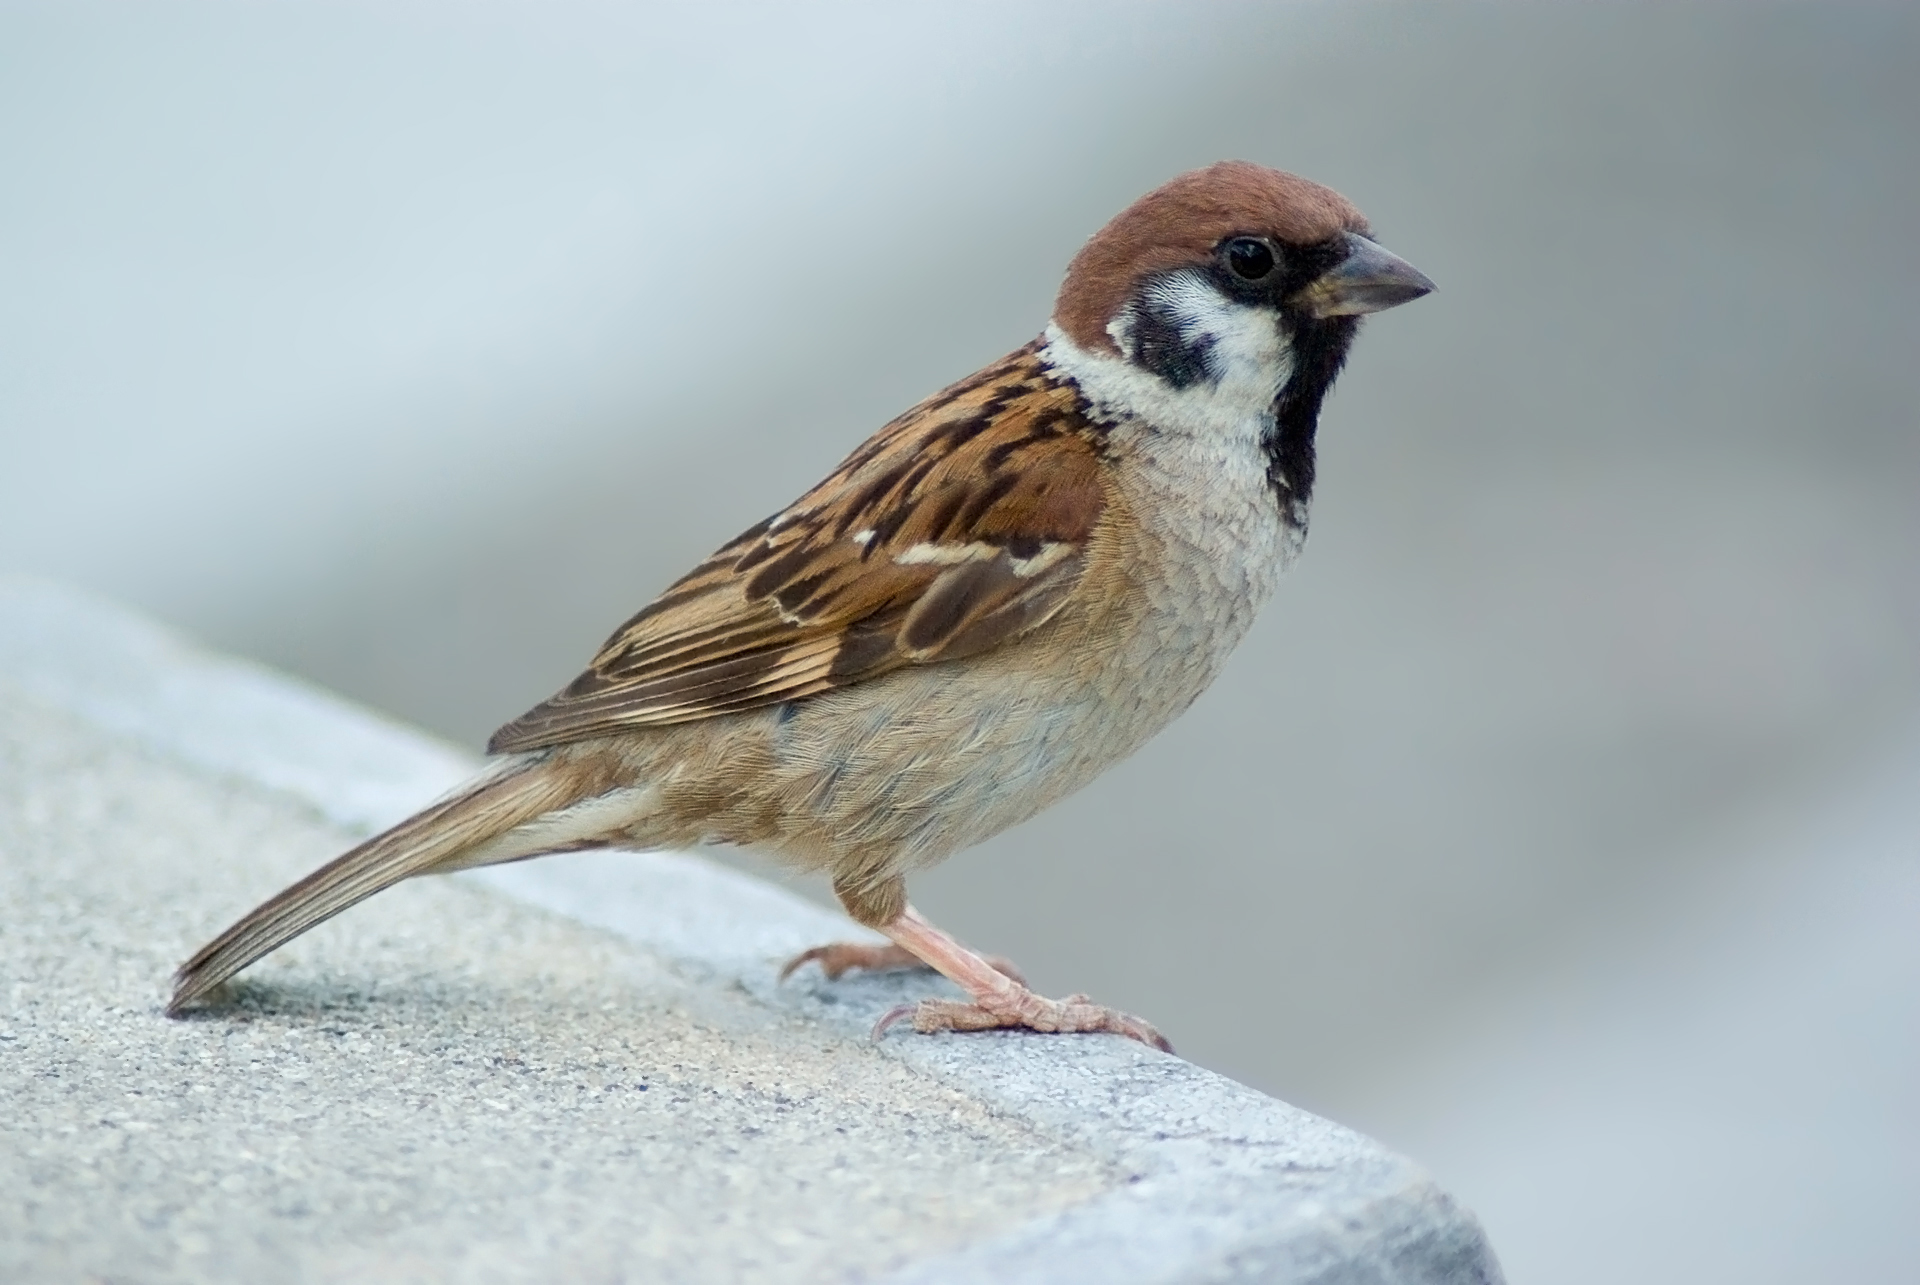
\includegraphics[width=0.4\textwidth]{\GRAPHPATH/spatz}}}$
    \onslide<+->
    \hspace*{0.025\textwidth}>\hspace*{0.025\textwidth}
    $\vcenter{\hbox{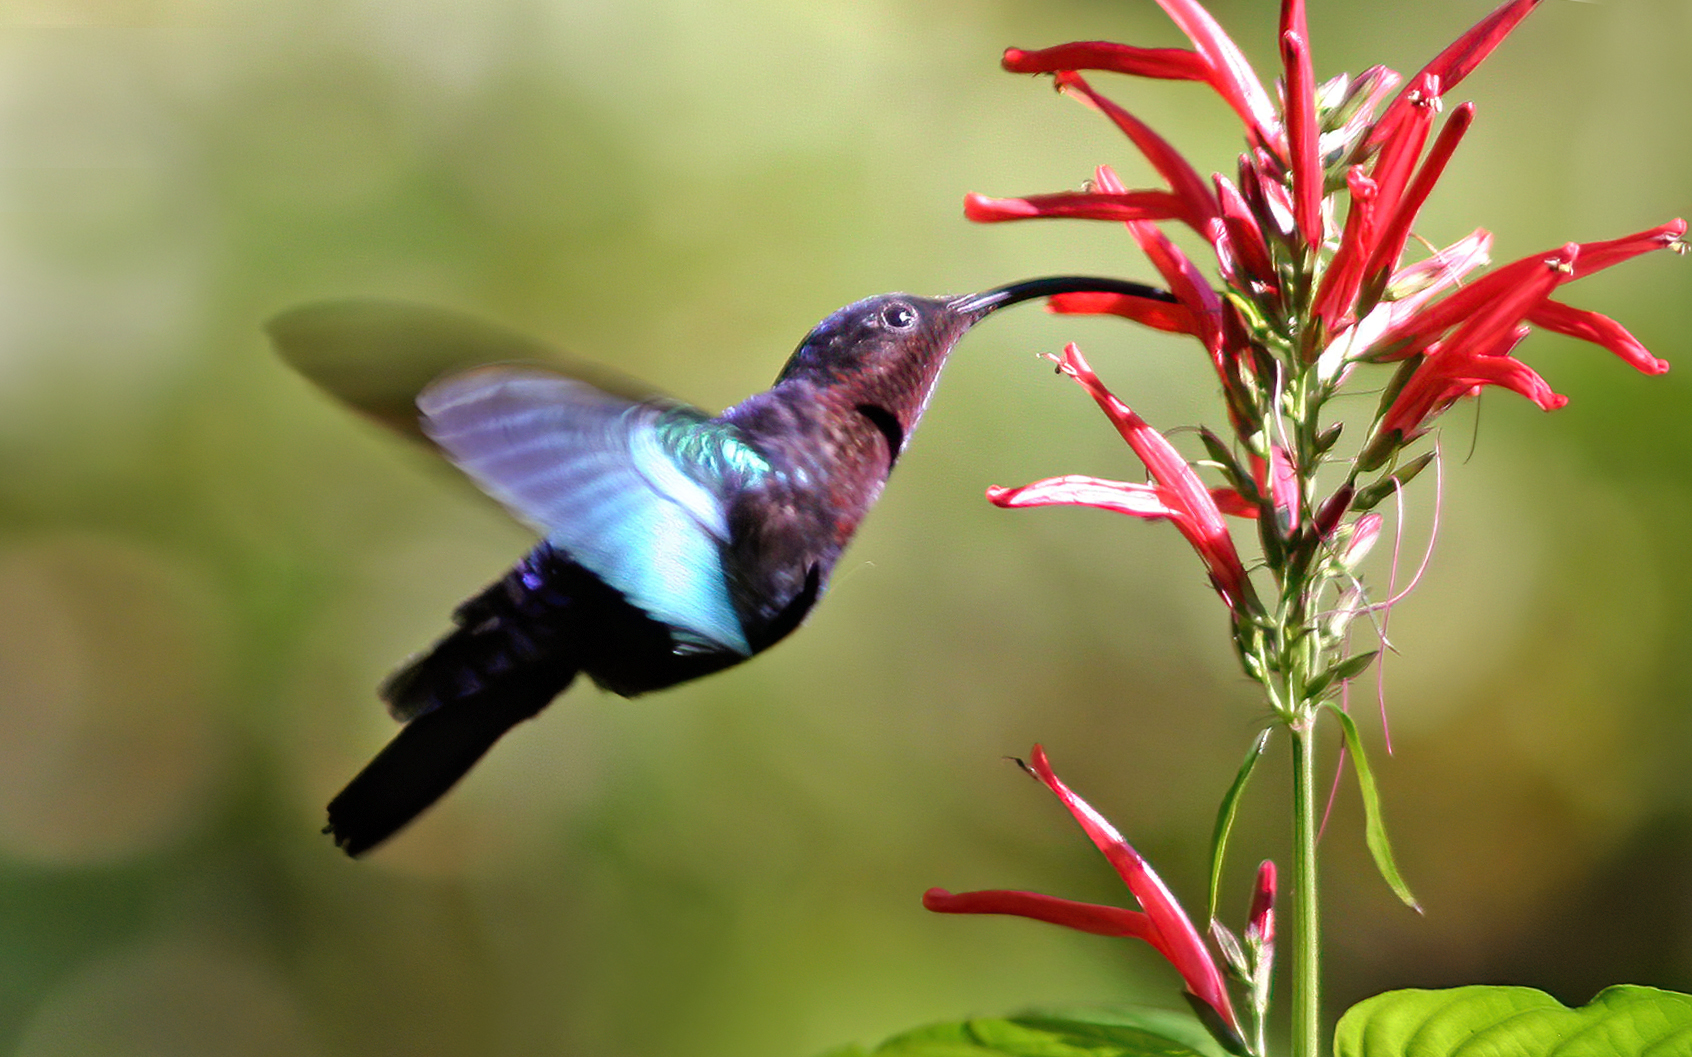
\includegraphics[width=0.25\textwidth]{\GRAPHPATH/kolibri}}}$
    \onslide<+->
    \hspace*{0.025\textwidth}>\hspace*{0.025\textwidth}
    $\vcenter{\hbox{\includegraphics[width=0.1\textwidth]{\GRAPHPATH/kiwi}}}$
  \end{minipage}\\
  \Halbzeile
  \centering 
  \grau{\tiny Bildquelle: Wikipedia}
\end{frame}

\begin{frame}
  {Programmatisches Schlussbild | Antwort}
  \onslide<+->
  \onslide<+->
  Die ewige Schwachsinnsfrage: Sind Kiwis und Pinguine nun \gruen{Vögel} oder nicht?\\
  \Viertelzeile
  \grau{Nur getoppt von: Erdbeeren sind gar keine Beeren, sondern Sammelnussfrüchte.}\\
  \Zeile
  \begin{itemize}[<+->]
    \item \alert{Kognition} | \orongsch{intrinsisch nicht diskret}, sondern ähnlichkeitsbasiert und \orongsch{parallel}
      \begin{itemize}[<+->]
        \item \orongsch{Netzwerkarchitektur}
      \end{itemize}
      \Halbzeile
    \item \alert{Symbole} = Phone, Morphe, Wörter, Phrasen, \ldots | \orongsch{intrinsisch} diskret und \orongsch{linear}
      \begin{itemize}[<+->]
        \item \orongsch{akustisches} Medium | Sagen Sie mal zwei Wörter gleichzeitig!
        \item \orongsch{schriftliches} Medium | Lesen Sie mal \textit{Zettels Traum} von Arno Schmidt\\
          \grau{(inkl.\ der Versuche, mehrere Wörter "`in einem"' zu schreiben)}
      \end{itemize}
    \Halbzeile
    \item[\ding{222}] Da wir nur akustisch oder über schriftliche Artefakte kommunizieren können,\\
      \alert{muss das Sprachsystem symbolisch sein}.
    \item[\ding{222}] Da es architekturbedingt nur nicht-symbolisch verarbeiten kann,\\
      \alert{muss das Gehirn symbolische Systeme so gut wie nötig und möglich emulieren}.
  \end{itemize}
\end{frame}


\begin{frame}
  {Programmatisches Schlussbild | Ausführung}
  \onslide<+->
  \onslide<+->
  Auch nicht-verschriftete Sprache muss medial bedingt logische Eigenschaften haben.\\
  \onslide<+->
  Kulturell bilden sich stärker symbolische Modi aus, vor allem durch Schrift.\\
  \grau{\footnotesize Norm, Selbst- und Fremdkorrektur, Textplanung, intensionale Definitionen, Explizierung, \ldots}\\
  \grau{\footnotesize Warum wird das vor allem im Kontext von Schule, Fremdsprache und Bildungssprache diskutiert?}\\
  \onslide<+->
  \Zeile
  \Halbzeile
  \centering 
  \begin{tabular}[h]{cc}
    \grau{(= spontane Sprachproduktion)} & \\
    \orongsch{weniger symbolische Eigenschaften} & \small \orongsch{informelle Alltagssprache} \\
    \onslide<+->
    \textcolor{orgrA}{\faArrowDown} &\large \textcolor{orgrA}{formelle Alltagssprache} \\
    \onslide<+->
    \textcolor{orgrB}{\faArrowDown} &\Large \textcolor{orgrB}{Bildungssprache} \\
    \onslide<+->
    \textcolor{orgrC}{\faArrowDown} &\LARGE \textcolor{orgrC}{Wissenschaftssprache} \\
    \onslide<+->
    \textcolor{orgrD}{\faArrowDown} &\huge \textcolor{orgrD}{Orthosprache} \\
    \onslide<+->
    \gruen{mehr symbolische Eigenschaften} & \gruen{\Huge formales System} \\
    \grau{(= reflektierte Sprachproduktion)}  & \\
  \end{tabular}
\end{frame}

\ifdefined\HANDOUT
  \begin{frame}
    {Und was ist denn nun mit Kiwis und Pinguinen?}
    \onslide<+->
    \onslide<+->
    Unser Verständnis der Welt führt zu genaueren und diskreten Kategorisierungen,\\
    \orongsch{wo dies nötig ist}. \alert{Die Sprache folgt dem erforderlichen Maß an Genauigkeit\slash Diskretheit.}\\
    \Zeile
    \onslide<+->
    \centering
    \begin{tikzpicture}
      \node at (0cm, 0cm) {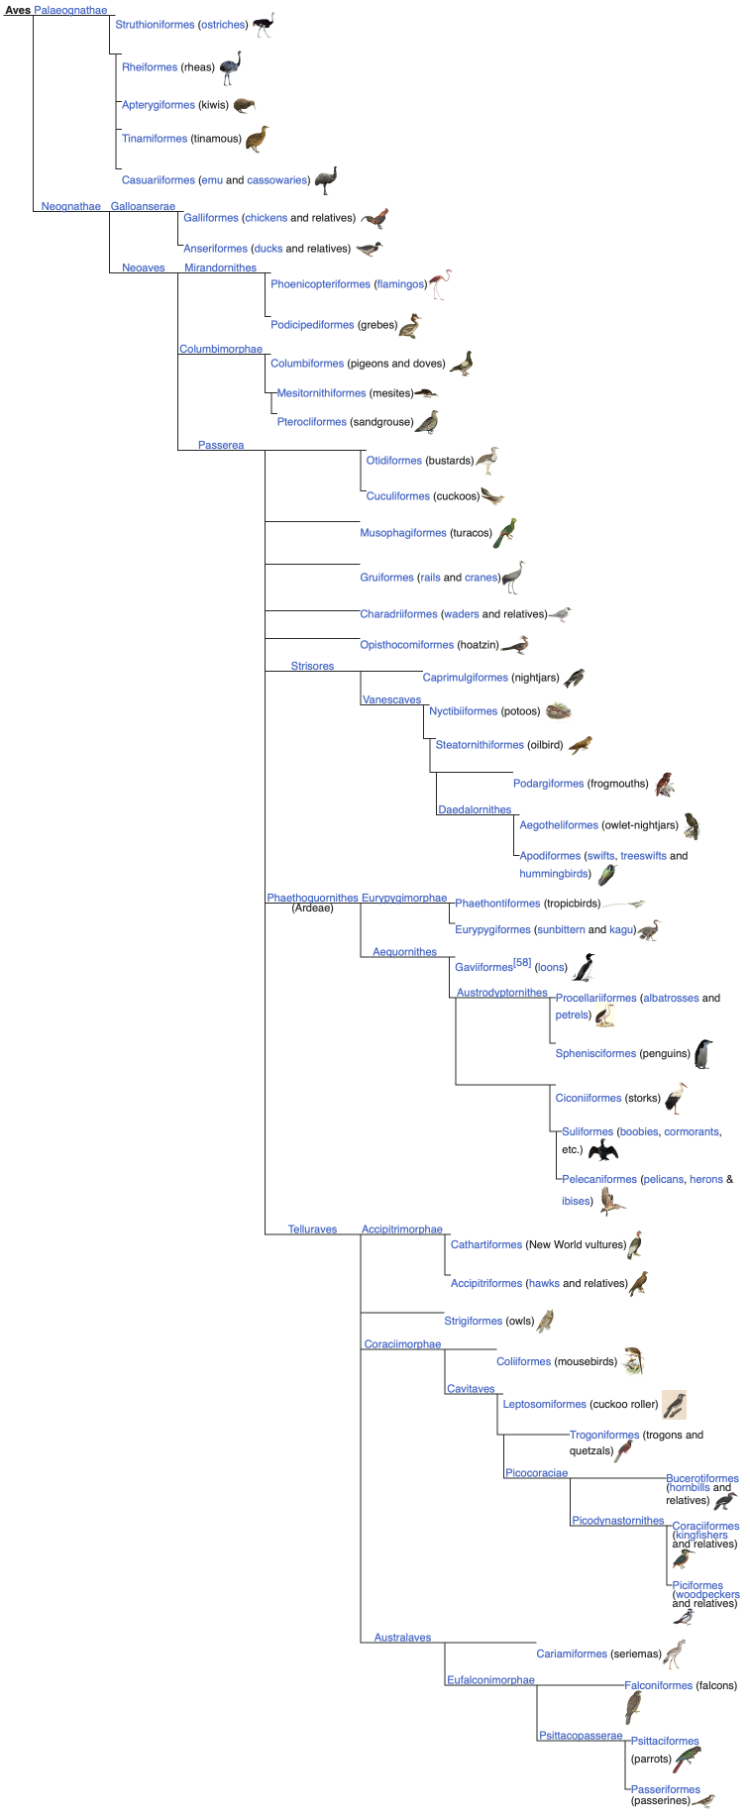
\includegraphics[height=0.6\textheight]{\GRAPHPATH/birds50}};
      \node at (5cm, 1.5cm) {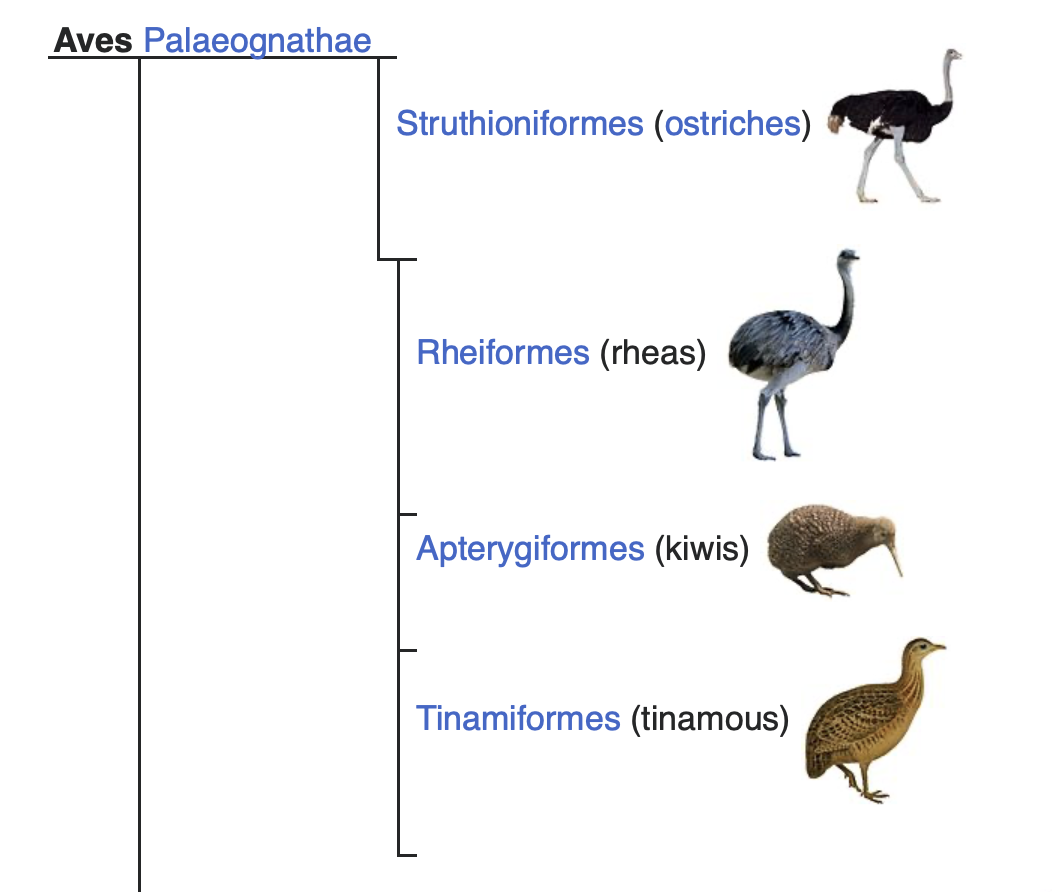
\includegraphics[height=0.25\textheight]{\GRAPHPATH/kiwis}};
      \node at (5cm, -1.5cm) {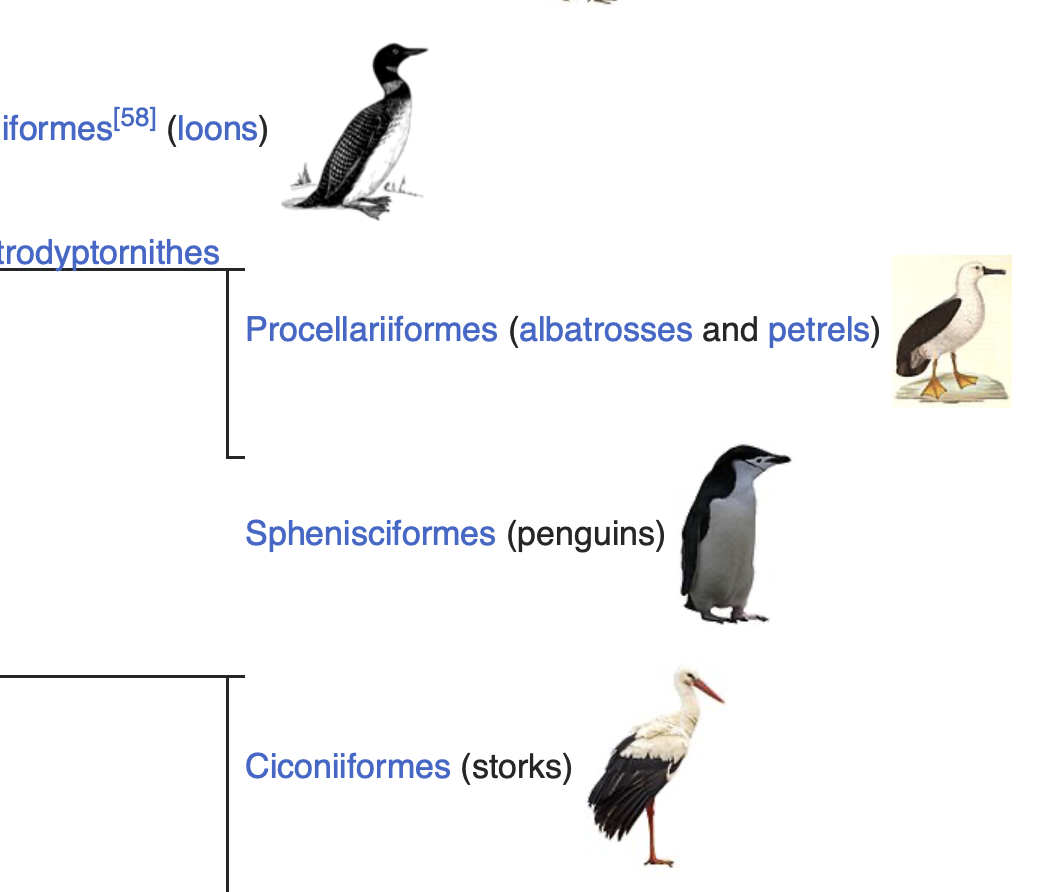
\includegraphics[height=0.25\textheight]{\GRAPHPATH/penguins}};
      \path (-0.3cm, 2.5cm) edge [-latex] (4.6cm, 1.25cm);
      \path (1.1cm, -0.45cm) edge [-latex] (4.2cm, -1.725cm);
    \end{tikzpicture}\\
    \Halbzeile
    \grau{\tiny Bildquelle: Wikipedia}
  \end{frame}
\else
  \begin{frame}
    {Und was ist denn nun mit Kiwis und Pinguinen?}
    \onslide<+->
    \onslide<+->
    Unser Verständnis der Welt führt zu genaueren und diskreten Kategorisierungen,\\
    wo dies nötig ist. \alert{Die Sprache folgt diesem Maß an Genauigkeit und Diskretheit!}\\
    \Zeile
    \onslide<+->
    \centering
    \begin{minipage}{0.9\textwidth}
    \centering
      $\vcenter{\hbox{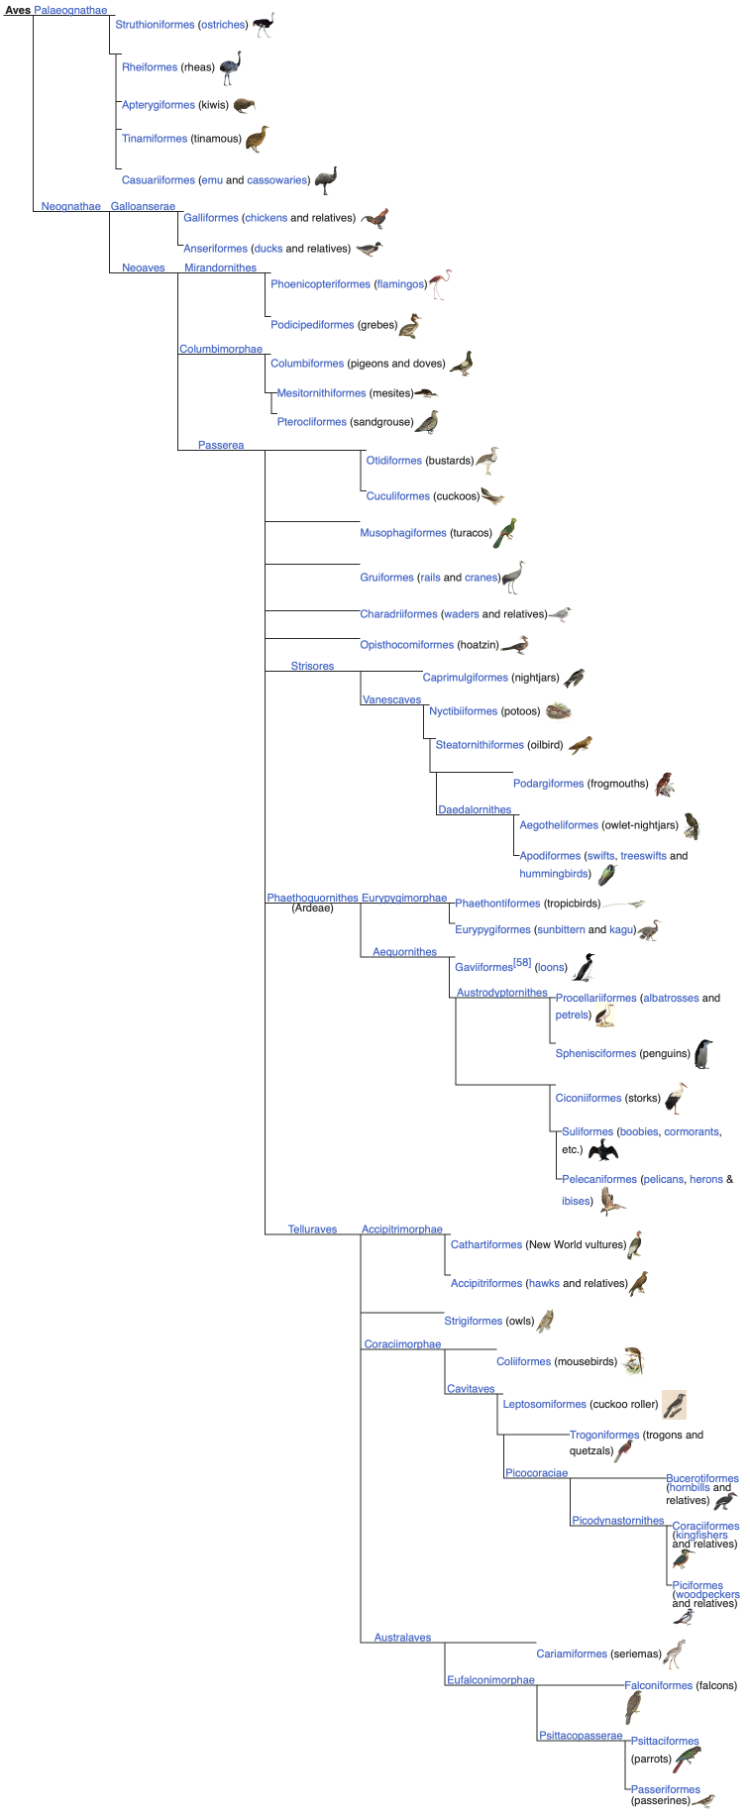
\includegraphics[height=0.7\textheight]{\GRAPHPATH/birds50}}}$\hspace{0.1\textwidth}
        \only<3>{$\vcenter{\hbox{\rule{0.4\textwidth}{0em}}}$}%
        \only<4>{$\vcenter{\hbox{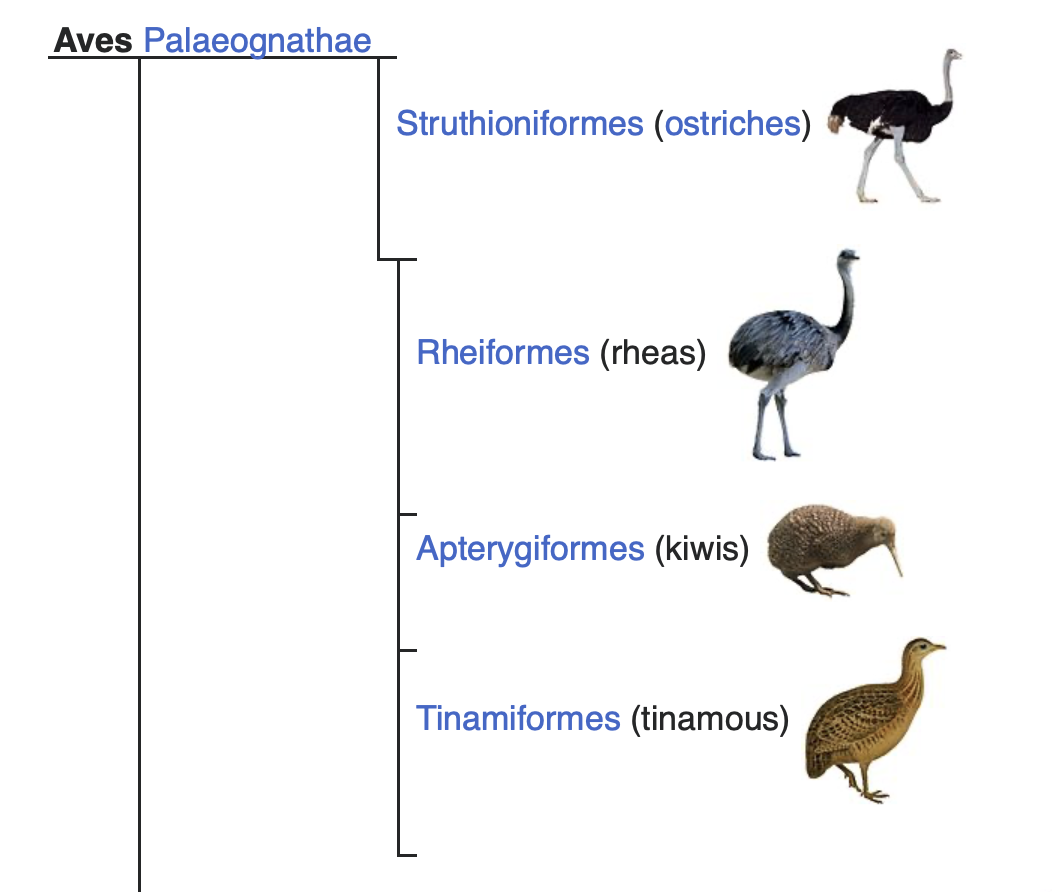
\includegraphics[width=0.4\textwidth]{\GRAPHPATH/kiwis}}}$}%
        \only<5>{$\vcenter{\hbox{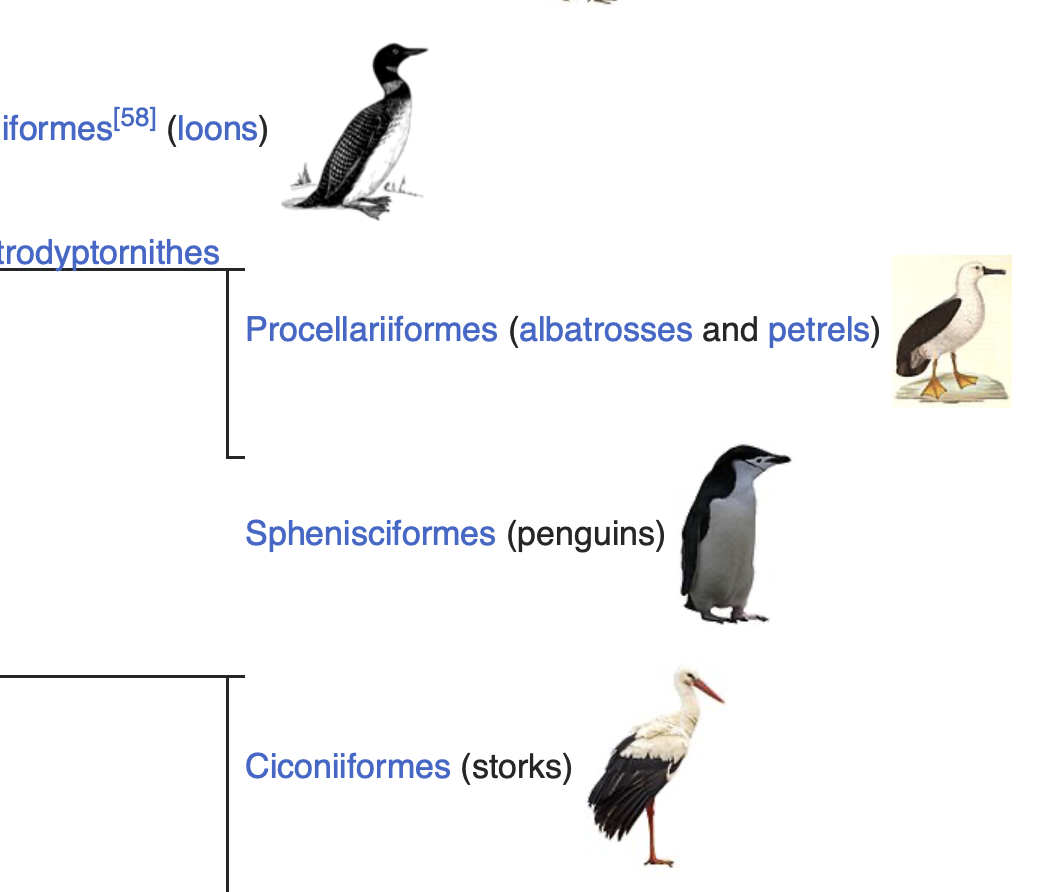
\includegraphics[width=0.4\textwidth]{\GRAPHPATH/penguins}}}$}
    \end{minipage}\\
    \grau{\tiny Bildquelle: Wikipedia}
  \end{frame}
\fi

\begin{frame}
  {Letzte Folie}
  \onslide<+->
  \begin{itemize}[<+->]
    \item Viele Missverständnisse in der Linguistik basieren darauf,\\
      dass das eben Gesagte nicht dem allgemeinen Forschungsprogramm zugrundeliegt.
    \item Die Doppelnatur von Sprache führt dazu, dass sowohl rein formale Linguistik\\
      und sogenannte kognitive Linguistik scheinbar erfolgreich sind.
    \item Im Prinzip läuft aber die Linguistik aktuell weitgehend ins Leere.
      \Halbzeile
    \item \alert{Modelltheoretische Semantik beschreibt einen essentiellen Teil von Sprache!}
    \item \alert{Sie modelliert logische Eigenschaften und den Bezug zur realen objektiven Welt.}
      \Halbzeile
    \item \small \grau{Ganz am Rande zu generativer AI:}
      \begin{itemize}[<+->]
        \item \grau{Erfolg | Sie modelliert völlig natürliche Grammatik.}
        \item \grau{Also alle traditionellen Grammatiker inkl.\ Chomsky: Setzen!}
        \item \grau{Gebrauchsbasiert ist generative AI sowieso. Also Stefan Gries: Setzen!}
          \Viertelzeile
        \item \grau{Misserfolg | Sie weiß nichts über die Welt im eigentlichen Sinn von \textit{Wissen}.}
        \item \grau{Wissen wird über die Verarbeitung eines immensen sprachlichen Inputs vorgetäuscht.}
        \item \grau{Es handelt sich um eine Art fancy Papagei.}
      \end{itemize}
  \end{itemize}
\end{frame}
